% Euclidean Handout Number Two Fall 2013
\documentclass{tufte-handout}

%\geometry{showframe}% for debugging purposes -- displays the margins

%%%% Packages to make things pretty
\usepackage{amsmath,amsthm}
\usepackage{booktabs}
\usepackage{graphicx}
\setkeys{Gin}{width=\linewidth,totalheight=\textheight,keepaspectratio}
\graphicspath{{graphics/}}
\usepackage{units}
\usepackage{fancyvrb}
\fvset{fontsize=\normalsize}
\usepackage{multicol}
\usepackage{pdfpages}

%%%% Theorem Evironments
\theoremstyle{definition}
\swapnumbers
\newtheorem{problem}{Problem}[section]
\newtheorem{conjecture}[problem]{Conjecture}
\newtheorem*{definition}{Definition}
\newtheorem*{theorem}{Theorem}
\newtheorem{question}[problem]{Question}
\newtheorem{challenge}[problem]{Challenge}
\newtheorem*{postulate}{Postulate}

%%%%%

\title{Euclidean Geometry:\\An Introduction to Mathematical Work}
\author[]{Math 3600, Fall 2013}
\date{7 September}

\begin{document}

\maketitle

\begin{marginfigure}
    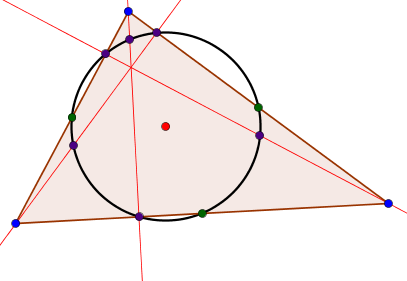
\includegraphics{NPC}
\end{marginfigure}

\setcounter{section}{11}
\section{Construction Problems}

The following problems are \underline{construction challenges}. In each case, you are to
\begin{compactenum}
\item find a compass and straightedge construction,
\item enumerate your steps, and
\marginnote{ A ``step'' for our counting purposes happens exactly every time you draw something with either the compass or straightedge.
We count steps using the modern ``fixable compass.''
This means that you may copy some segment length for the radius of a circle, but place it at a new point for a center all in one step.
If you like, this collapses the content of Euclid Proposition I.2 in to a single step.}
\item prove that your construction works.
\end{compactenum}
You may use any parts of the \emph{Elements} Book I.1-34 or Book III.1-34 as part of your reasoning.



For most challenges, I have included a ``par value" indicating the number of steps an experienced constructor would need.
Can you meet this or do better?


\begin{challenge}\label{chal:angle-bisector}
Given an angle, construct the angle bisector. (par 4)
\end{challenge}

\begin{challenge}\label{chal:midpoint}
Given a segment, find the midpoint. (par 3)
\end{challenge}

\begin{challenge}\label{chal:perp-pt-not-on-line}
Given a line $\ell$ and a point $A$ not lying on $\ell$, construct a line perpendicular to $\ell$ through $A$. (par 4, possible in 3)
\end{challenge}

\begin{challenge}\label{chal:perp-pt-on-line}
Given a line $\ell$ and a point $A$ lying on $\ell$, construct a line perpendicular to $\ell$ through $A$. (par 4, possible in 3)
\end{challenge}

\begin{challenge}\label{chal:copy-angle}
Given an angle at a point $A$ and given a ray emanating from a point $B$, construct an angle at $B$ congruent to the angle at $A$ having the given ray as a side. (par 4)
\end{challenge}

\begin{challenge}\label{chal:parallel}
Given a line $\ell$ and a point $A$ not lying on $\ell$, construct a line parallel to $\ell$ which passes through $A$. (par 3)
\end{challenge}

\begin{challenge}\label{chal:circle-center}
Given the circumference of a circle, find the center of the circle. (par 5)
\end{challenge}

\begin{challenge}\label{chal:tangent-circle-point}
Given a circle with center $O$, and given a point $A$ outside the circle, construct a line $\ell$ through $A$ which is tangent to the circle. (par 6)
\end{challenge}

\vfill
\end{document}

%sagemathcloud={"zoom_width":100}